\section{Vulnerability: Login always as user 0}
\label{sec:background}
\textbf{Description:} Upon logging into the website as the second user I had created, \textit{hacker@wondoughbank.com}, it became clear that the transactions displayed were in fact
not belonging to the user \textit{hacker@wondoughbank.com}. It was then immediately clear that they belonged to the original user \textit{intern@wondoughbank.com}. This was confirmed
when it was observed that the tokens created were all associated with the user whose id was 0.
\begin{figure}[h]
   \centering
   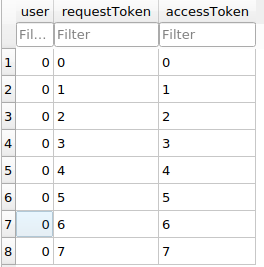
\includegraphics[width=0.5\textwidth]{figs/token1.png}
   \caption{The table of tokens showing each was associated with the user 0}
   \label{fig3}
 \end{figure}\\
This would allow all users access to user 0's account. This is a critically important vulnerability since it could be accidentally exploited by well meaning users as well as hackers.
It is also a vulnerability that requires no technical knowledge to exploit and this low skill ceiling makes it of particular threat. If combined with the fact that the bank used
to allow the transfer of money from one account to another, attackers could transfer unlimited money easily from the account of the unfortunate user whose id happens to be 0.\\ \\
\textbf{Testing the Vulnerability:} I tested this vulnerability as a hacker would by simply logging in as user 1 (which would then naturally log me in as user 0) and then
transferring money to user 1. I watched the money leave my account, which proves the issue since transferring money to myself should cause no change in value to my balance.
This would be how a hacker could exploit such a vulnerability but also how a regular user simply not paying attention and thinking they had logged into their account could also
cause trouble. This could make the vulnerability a further threat since an attacker could simply use this as an excuse if they were ever discovered to have used the attack.\\ \\
\textbf{Mitigation:} By using print lines in the \verb|getUSer()| function I discovered the issue. In the below code ids 1 and 2 in lines 1 and 2 returned 1, the correct id. This
meant that the issue was not in the fetching of the id from the database. Whilst id 3 printed 0 meaning the issue occured in the creation of the new user from the values from
the database.
\begin{minted}{java}
   System.out.println("\nID1"+rs.getInt(1));
   System.out.println("\nID2"+rs.getInt("id"));
   WondoughUser user = new WondoughUser(rs.getInt("id"),
       rs.getString("username"));
   user.setHashedPassword(rs.getString("password"));
   user.setSalt(rs.getString("salt"));
   user.setIterations(rs.getInt("iterations"));
   user.setKeySize(rs.getInt("keySize"));
   System.out.println("\nID3"+user.getID());
   return user;
\end{minted}
It then transpired that passing the id into the constructor of \verb|WondoughUser| was pointless since the constructor never set the value. Therefore I added the following line
to fix the issue. This is the user the tokens are created from and much more causing the root of the issue.
\begin{minted}{java}
   public WondoughUser(int id, String username) {
       this.username = username;
       this.id = id;//added line
   }
\end{minted}
From here I devised an automated test to call the \verb|getUser| command to test that the user returned shared the username and id of the functions parameters.